\documentclass[tikz,border=5pt]{standalone}
\usepackage{luatexja}
\usepackage[hiragino-pron]{luatexja-preset}
\usepackage{amsmath,amssymb}
\usepackage{pgfplots}
\pgfplotsset{compat=1.18}
\usetikzlibrary{arrows.meta,calc,decorations.markings,patterns,positioning}

% Common styles
\tikzset{
  axis/.style={-{Stealth[length=6pt]}, thick},
  curve/.style={thick, red},
  dashed curve/.style={thick, dashed, blue},
  dot/.style={circle, fill, inner sep=1.5pt},
  open dot/.style={circle, draw, fill=white, inner sep=1.5pt},
}

\begin{document}
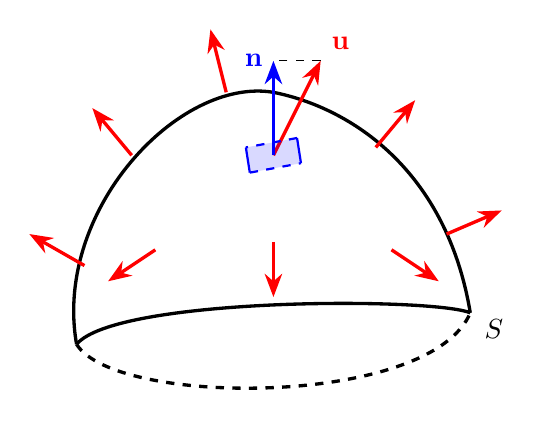
\begin{tikzpicture}[>=Stealth, thick]

  % Surface S (dome shape, asymmetric blob)
  \draw[very thick]
    (-2.5,-0.2) .. controls (-2.8,1.5) and (-1.2,3.2) .. (0,3.0)
    .. controls (1.0,2.8) and (2.2,2.0) .. (2.5,0.2);

  % Bottom ellipse (dashed back, solid front)
  \draw[very thick, dashed] (-2.5,-0.2) .. controls (-2.0,-1.0) and (2.0,-1.0) .. (2.5,0.2);
  \draw[very thick] (-2.5,-0.2) .. controls (-2.0,0.4) and (2.0,0.4) .. (2.5,0.2);

  % Red outward normal arrows at various surface points
  \draw[->, red, very thick] (-2.4,0.8) -- ++(-0.7,0.4);
  \draw[->, red, very thick] (-1.8,2.2) -- ++(-0.5,0.6);
  \draw[->, red, very thick] (-0.6,3.0) -- ++(-0.2,0.8);

  \draw[->, red, very thick] (1.3,2.3) -- ++(0.5,0.6);
  \draw[->, red, very thick] (2.2,1.2) -- ++(0.7,0.3);

  % Red outward normal arrows on the front side of the surface
  \draw[->, red, very thick] (-1.5,1.0) -- ++(-0.6,-0.4);
  \draw[->, red, very thick] (0.0,1.1) -- ++(0.0,-0.7);
  \draw[->, red, very thick] (1.5,1.0) -- ++(0.6,-0.4);

  % Black arrow: vector field u at point P (tilted, with vertical component = blue n)
  \coordinate (P) at (0.0,2.2);
  \draw[->, red, very thick] (P) -- ++(0.6,1.2) node[above right] {$\mathbf{u}$};
  % Dashed projection line from tip of u down to tip of n
  \draw[dashed, thin] (0.6,3.4) -- (0,3.4);

  % Blue normal vector n = vertical component of u
  \draw[->, blue, very thick] (P) -- ++(0,1.2) node[left] {$\mathbf{n}$};

  % Blue dS parallelogram at P
  \coordinate (dA) at (-0.3,-0.22);
  \coordinate (dB) at (0.35,-0.1);
  \draw[blue, thick, dashed]
    ($(P)+(dA)$) -- ($(P)+(dB)$)
    ($(P)-(dA)$) -- ($(P)-(dB)$);
  \draw[blue, thick]
    ($(P)+(dA)$) -- ($(P)-(dB)$)
    ($(P)-(dA)$) -- ($(P)+(dB)$);
  \fill[blue, opacity=0.15]
    ($(P)+(dA)$) -- ($(P)+(dB)$) -- ($(P)-(dA)$) -- ($(P)-(dB)$) -- cycle;

  % S label
  \node at (2.8,0.0) {$S$};

\end{tikzpicture}
\end{document}
